%
%  Appendix : PIC
% ================
%

\chapter{Particle in Cell (PIC)}
\label{Apx:PIC}

The Particle in Cell method (PIC) is a numerical technique to solve a certain class of partial differential equations.
Particles are usually represented by macro particles, that is, one virtual particle in the simulation represents multiple real particles.
The particles are tracked in continuous phase space, and they interact only through average fields.
Moments of the distribution function are computed simultaneously on a Eulerian mesh to solve the self-consistent field equations~\cite{hatzky:2010}.
PIC codes can be electrostatic or electromagnetic.
Both PIC codes used in this work are electromagnetic, so we will only cover that approach.

Most of the work presented in this thesis was done using OSIRIS~\cite{fonseca:2002, add:fonseca:2017}.
OSIRIS is a fully relativistic and parallelised 3D PIC code.
It is written in an object-oriented style with Fortran 90.

For the concluding paper, we opted to instead use QuickPIC~\cite{an:2013, huang:2006} as the main simulation tool, although preliminary simulations were done using OSIRIS.
QuickPIC is a quasi-static PIC code, which was better suited for emittance studies as the full PIC method suffers from instabilities that proved to significant for that study.

This Appendix will briefly outline some of the properties of the PIC method, but limited to what is relevant for the work presented and the simulation codes used.

% ================================================================================================================================ %
\section{The Full Electromagnetic PIC Method}
\label{PIC:EM}

The main steps involved in the Electromagnetic PIC method are outlined in Figure~\ref{Fig:PIC}.
This method is solved on a grid using Maxwell's equations
\begin{align}
    &\nabla\cdot\vec{E}  = \frac{\rho}{\epsilon_0} \\
    &\nabla\cdot\vec{B}  = 0 \\
    &\nabla\times\vec{E} = -\frac{\partial\vec{B}}{\partial t} \\
    &\nabla\times\vec{B} = \mu_0\left(\vec{J} + \epsilon_0\frac{\partial\vec{E}}{\partial t}\right),
\end{align}
while the particles are advanced in time using the Newton-Lorentz equations
\begin{align}
    \frac{\mathrm{d}x}{\mathrm{d}x} &= \vec{v} \\
    \frac{\mathrm{d}(\gamma x)}{\mathrm{d}x} &= \frac{q}{m}\left(\vec{E}+\vec{v}\times\vec{B}\right).
\end{align}

The charge density $\rho$ and current density $\vec{J}$ are interpolated onto the grid from the particle positions and velocity respectively, while the electric and magnetic fields are interpolated onto the particles when updating their position and velocity~\cite{vay:2016}.

\begin{figure}[hbt]
    \centering
    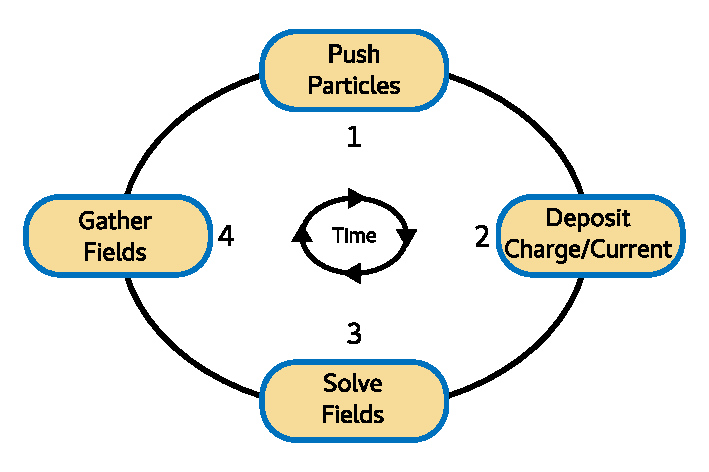
\includegraphics[width=0.7\linewidth]{figures/PIC-Diagram}
    \caption{\label{Fig:PIC}
        The four main steps of the PIC algorithm.
        1: Evolve the velocity and position of the particles using the Newton-Lorentz equations.
        2: Interpolate and deposit the charge/current densities onto the grid.
        3: Evolve the Maxwell's equations, or Poisson's equation if electrostatic.
        4: Interpolate the fields from the grid onto the particles for the next push.
        Recreated from Vay \etal~\cite{vay:2016}.
    }
\end{figure}

\begin{description}
    \item[Step 1 -- Particle Push:] The Newton-Lorentz equations can be discretised with a centred finite difference discretisation, such that
    \begin{align}
        \frac{\vec{x}^{i+1} - \vec{X}^i}{\Delta t} &= \vec{v}^{i+1/2} \\
        \frac{\gamma^{i+1/2}\vec{v}^{i+1/2} - \gamma^{i-1/2}\vec{v}^{i-1/2}}{\Delta t} &=
            \frac{q}{m}\left(\vec{E}^1 + \vec{v}^i \times \vec{B}^1\right).
    \end{align}
    This requires that $\vec{v}^i$ can be represented by the known quantities, to which the Boris' method provides a very efficient second-order accurate and time reversible solution outlined in a 1970 paper \cite{boris:1970}.
    However, this method is not Lorentz-invariant \cite{vay:2008} making it unsuitable for ultra-relativistic applications.
    Lorentz-invariance can be achieved by substituting a velocity average in place of a single-step velocity calculation.
    This, however, comes with a performance penalty.
    For further details and derivations of the different methods, see \cite{vay:2016} and therein cited references.
    
    \item[Step 2 -- Charge and Current Deposition:] The charge and current can be deposited on the grid using various interpolation methods \cite{abe:1986}.
    The densities are deposited from the particle position and velocities using an interpolation $S$,
    \begin{align}
        \rho    &= \frac{1}{\Delta x \Delta y \Delta z} \sum_n q_n S_n \\
        \vec{J} &= \frac{1}{\Delta x \Delta y \Delta z} \sum_n q_n \vec{v}_n S_n.
    \end{align}
    Accumulation of errors resulting from violation of Gauss' law by the discretisation need to be prevented.
    This can be achieved by either modifying the deposition to prevent such violations, or by using methods that are exact when combined with the field solver in step 3 \cite{vay:2016}.
    OSIRIS makes several interpolation methods available to the user, with varying level of performance and accuracy.
    
    \item[Step 3 -- Field Solver] There are many implementations of field solvers for PIC codes, and OSIRIS supports multiple such methods.
    The most relevant here, and the OSIRIS default, is the Yee solver \cite{yee:1966}.
    The Yee solver uses a staggered grid where the electric field components are located between nodes. while the magnetic field components are located at the centre of the grid cell faces.
    This is illustrated in Figure~\ref{Fig:PIC:EMF}.
    The time integration of the fields is done using alternate half time-step leaps, also known as the \textit{Leapfrog} integration scheme.
    Other solvers not covered here are outlined in \cite{vay:2016}, some of which are also available in OSIRIS.
    
    \item[Step 4 -- Gather Fields:] The fields are gathered from the grid and onto the macro particles, usually through the same interpolation $S$ as used in Step 2.
    This is generally done through a scheme tuned to conserve either energy or momentum.
\end{description}

\begin{figure}[hbt]
    \centering
    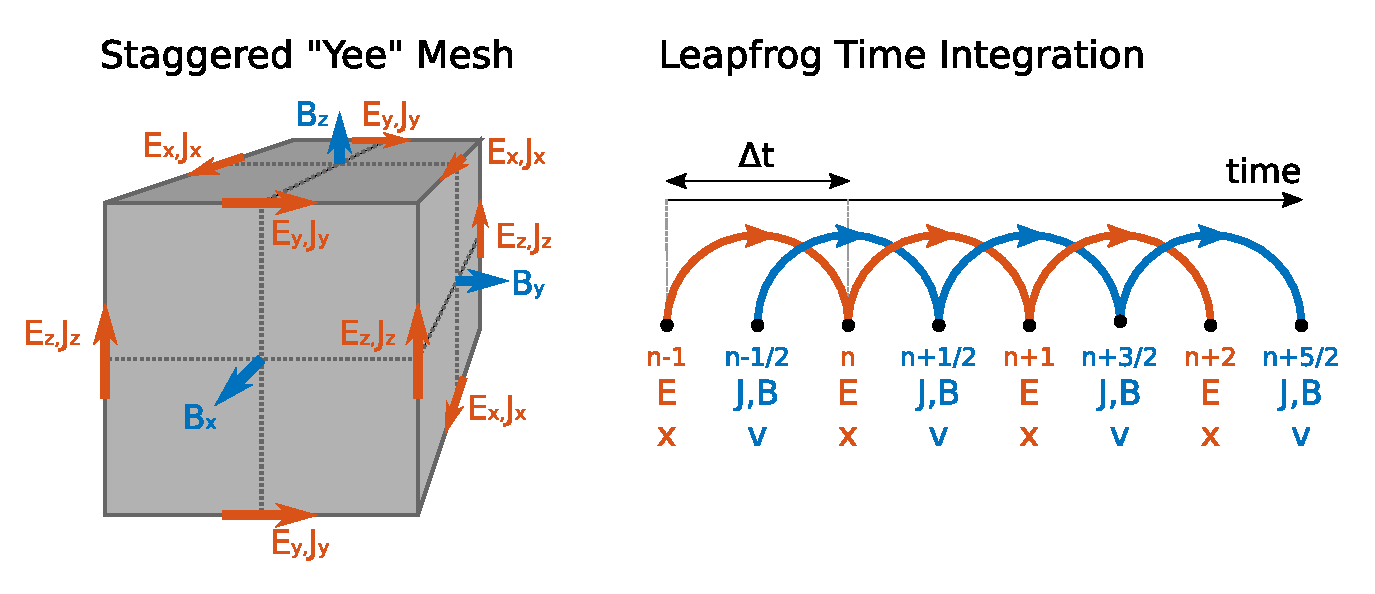
\includegraphics[width=0.75\linewidth]{figures/EMFSolver}
    \caption{\label{Fig:PIC:EMF}
        \textbf{Left:} The staggered Yee grid. Current densities and electric fields are defined on the edges of the cells, and magnetic fields on the faces.
        \textbf{Right:} Leapfrog time integration uses alternating half time steps for electric and magnetic fields.
        Recreated from Vay \etal~\cite{vay:2016}.
    }
\end{figure}

This method is computationally heavy as all the particle species that make up the plasma accelerator need to be simulated.
This includes the electrons and possibly ions that makes up the plasma.
In most cases the ions can be assumed to be stationary, and can thus be replaced by a static background charge density.
However, OSIRIS does have the ability to simulation ions as well as ionisation of a neutral gas if necessary.

A common way to reduce the computational cost is to only simulate the region populated by the propagating beams using both a moving window in a Lorentz-boosted frame.
The latter significantly reduces the number of time steps needed by up to $\approx (i+\betar)\gammar^2$~\cite{vay:2011}.

% ================================================================================================================================ %
\subsection{Numerical Cherencov}
\label{PIC:NumCher}

Relativistic PIC codes nearly universally suffer a well understood numerical instability known as \textit{Numerical Cherenkov}.
This issue arises with finite difference time domain algorithms like the Yee solver, and is caused by an anisotropic numerical phase error.
The result of this is that the numerical phase velocity is slower than the physical phase velocity of the fields for some modes.
It is in addition both frequency dependant and time resolution dependant~\cite{godfrey:1974, greenwood:2004}.
This implies that it can be managed in many cases by limiting its impact by paying close attention to the time resolution of the simulation as well as ensuring a good grid resolution.
However, this is not always cost effective in terms of computing power.

The consequence of this numerical instability is that it induces emittance growth in simulations with high charge density witness bunches.
The problem can be somewhat mitigated by filtering or dampening high-frequencies.
However, this inevitably has an impact of the physics.
The problem can also be mitigated by modifying the discretisation of the Maxwell equations such that one can choose a $\Delta t = \Delta x/c$~\cite{pukhov:1999}.
This scheme, however, triggers numerical oscillations around the Nyquist frequency $k = \pi/\Delta x$~\cite{vay:2011a}.

Other methods were developed to prevent Numerical Cherenkov without the $\delta t = \Delta x/c$ criterion, but which requires an isotropic grid, limiting practical applications~\cite{greenwood:2004}.
This method modifies the Yee grid by taking into account the fields another grid layer out from the cell being computed, in order to better approximate the curl of the field at high frequency.
There most recent scheme is the Lehe solver, based on a 2013 paper, which is a modification the isotropic grid solver, but which is adapted for an anisotropic grid~\cite{lehe:2013}.
OSIRIS~3.0 implements a version of this solver.

% ================================================================================================================================ %
\section{The Quasi-Static Electromagnetic Method}
\label{PIC:QS}

The quasi-static approximation takes advantage of the fact that a beam travelling close to the speed of light is very rigid, and therefore responds slowly, while the plasma response is very fast in comparison.
This separation of response in time scale allows a separation in how these components of the simulation are treated.

While the particle bunches are simulated in 3D, the plasma is simulated in 2D slices.
The response of the plasma can then be computed slice by slice as the particle bunches pass through them.
This can in fact be done in parallel very efficiently.
The longitudinal and transverse structure of the wake can then be constructed from the slices of plasma, and a complete electromagnetic field map computed.
This can then be applied to the macro particles to evolve their position and velocity.

There are several ways to perform the necessary calculations, and each implementation of the method may have different solutions.
Some key details are outlined in \cite{vay:2016}.

\bigskip
\noindent\textbf{For example:}
\bigskip

In QuickPIC, the plasma particle trajectories are parametrised with $[x(\xi), y(\xi), s(\xi)]$, while the beam particles are parametrised with $[x(s),y(s),\xi(s)]$, where $\xi = ct - z$ is the simulation window coordinate and $s=z$ is the position along the simulation.
The variables $\xi$ and $s$ have the same unit, but correspond to the two different time scales, fast and slow respectively~\cite{huang:2006}.
This approximation implies that for short bunches, $s$ is the same for all plasma particles, reducing the plasma particle motion to movement in the $x,y$-plane.
At the same time the beam evolves very slowly and with respect to $s$, compared to the fast plasma response on the plasma wavelength scale of the coordinate $\xi$.
When solving the field equations it is thus assumed that $\partial/\partial s = 0$, meaning the corresponding first and second derivative terms can be dropped~\cite{an:2013}.
The charge and current densities for the beam are deposited onto the grid in the same way as with the full PIC method.

The flow of the QuickPIC algorithm is slightly different than presented for full PIC in Figure~\ref{Fig:PIC}.
While the main loop is 3D, a 2D loop is embedded inside it.
After initialisation, the 3D loop hands the token over to the 2D loop which initialises new slices of plasma, runs its field solver, pushes the plasma particles, and deposits onto the grid.
The token is then passed back to the 3D routine which pushes the beam particles, and deposits the charge and current of these onto the grid, before returning to the start of the 3D loop again.
For a full review of the flow and the numerical implementation of each of the steps, see Huang \etal~\cite{huang:2006}.

% ================================================================================================================================ %
\section{Considerations}
\label{PIC:Full}

OSIRIS~3.0 initialises all fields at zero, meaning that a certain amount of simulation time steps are required in order for the fields to build up to their proper values.
Typically, simulations let the bunches drift for a few millimetres or centimetres in vacuum before the plasma is introduced.
To prevent evolution of the bunches during this stage, it is possible to either ramp up their charge, or their energy while preventing the bunch from transverse evolution.

QuickPIC allows the user to specify initial emittance of the bunch as well as its spatial distribution.
The bunch is initialised at waist, that is the Twiss parameter $\alpha = 0$ (see Section~\ref{Int:BPI:EnTwiss}).
OSIRIS~3.0 does not provide an input option for emittance, but it does allow the user to specify a thermal distribution of particles as well as their fluid momentum.
The thermal distribution, which is by default Gaussian, can thus be used to specify a transverse momentum distribution that is uncorrelated by the spatial distribution.
This provides a way to control the initial bunch emittance at waist.
Evolution of the Twiss parameters during the above mentioned drift phase is effectively prevented by one of the two methods available to ramp the bunch which also freezes their transverse evolution.
